\documentclass[../main.tex]{subfiles}
\begin{document}
\chapter{Results}
\label{chap:resconc}

\section{Caveats}

Many difficulties connected with this research results from the fact that almost all the documents produced by the \textbf{RTCA}, the \textbf{EUROCAE} and the \textbf{ICAO} are paying products and every document ranges between 300 and 500 dollars. Therefore every necessary information had to be acquired in an alternative way: either by conferences slides, papers or articles.

Regarding \textit{dump1090} the extracted binaries they behave differently than expected: the one from FlightRadar24 does not print out any information on screen but it is heavily modified to upload data directly inside their network. On the other hand the binary extracted from the Stratux image have a strange behavior since, if fed with the \textit{1090\_small.bin} data file and given the \textit{-{}-no-crc-check} option it correctly outputs messages with CRC errors while the version from the \textit{Antirez} repository, which is supposed to be the same as the extracted one, when the same file and parameters are used it does not show such messages.

Working with the Unicorn Engine was not easy nor straight forward as this emulator is really powerful and well developed however it comes with no documentation at all but just a couple of C or Python very basic examples. Therefore, every time that more details where needed it was necessary to take a look at the source code and understand the functioning. Moreover, even if Unicorn is capable of emulating the ARM architecture in almost all his functionalities it does not have default support for Vector Floating Point (VFP) instructions which are widely used in the tested binary. As a consequence, the emulator was not able to recognize VFP instructions which resulted in a crash of the template that was in execution, following the ARM documentation it was possible to create a piece of code to enable VFP as in Figure \ref{fig:vfp}.

\begin{figure}[htp]
  \centering
  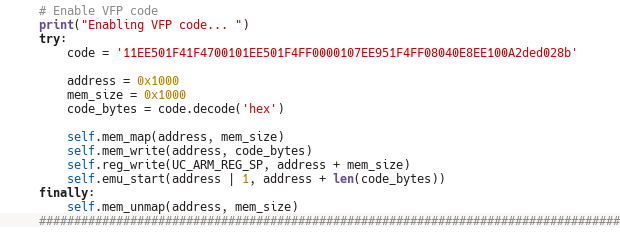
\includegraphics[scale=0.9]{images/vfpcode.png}
  \caption{Portion of python code to enable VFP instructions}
  \label{fig:vfp}
\end{figure}

Even after the emulator was able to run VFP instructions a lot of debugging was needed to make a single template work as it is quite common to have illegal memory access also in relation to library functions such as \textit{puts, printf, etc} that needs to be properly handled.

In addition to this \textit{afl-unicorn} was developed as an internal research project in a cybersecurity company, it is a great tool but there is little to no documentation on his functioning and more important there is no real walktrought on how to properly create a template for a binary. This is not a real problem since everything is clearly explained in the blog post about \textit{afl-unicorn} and in the basic template provided. Having to "work your way" through the tool is a great way to understand how it works but it requires quite a lot of time.

\textbf{AFL} had problems in finding crashes on the analyzed software and, in some case, even in the intentionally vulnerable binaries. This can be caused by many factors:

\begin{enumerate}

  \item The used test input was not good enough therefore it will require ages for \textbf{AFL} to generate an input capable of triggering the vulnerability, this is also supported by the extremely low and slow growing code coverage obtained during the tests.

  \item The vulnerability was actually triggered but the overflow did not caused any crash, therefore resulting in a corrupted zombie program that might
  never crash. Moreover, \textbf{AFL} cannot detect memory leaks and other type of corruptions in the program even though those are very likely security bugs.
  This type of problems is quite common in embedded devices as it has been widely detailed and analyzed in~\cite{corrcrash}.

  \item It is possible that the code object of test is written with security in
  mind and therefore no bugs are present in the code. The original author of
  \textit{dump1090}, Salvatore Sanfilippo\footnote{\url{http://invece.org/}}, has a strong security background and this might have influenced the security of code. However, the programs that we have tested are not the one used in the real embedded systems in airplanes, such systems can even have worst implementations of the protocols.

  \item Even if \textbf{AFL} represents the current state of the art in terms of binary fuzzing it might not be the right tool to use in this situation.

\end{enumerate}

As already mentioned acquiring data for \textit{dump978} was a trivial process since it is not used in Europe. Moreover, \textit{extract\_nexrad} does not implement any function to use Huffman encoding which was the most priomising part since it is likely to be vulnerable. The sample FIS-B (text and image) data acquired from the GDL90 document~\cite{gdl90} are not correctly decoded either by \textit{extract\_nexrad} and by \textit{uat2text}, further investigation discovered that there has been at least 2 revisions of the \textbf{RTCA} documents , such as RTCA DO-267A, that introduced changes in APDUs and packet formats. Some of those modifications, that are adopted in Europe under particular documents \acrlong{etso} (ETSO), are detailed in the ETSO-C157a from \acrlong{easa} (\textbf{\acrshort{easa}}) \cite{easa-all-etso}. ETSO-C157a has been introduced on 05/07/2012 and replaced on 16/12/2016 by ETSO-C157b which introduced further modifications.

These revisions brings some questions on how real avionics components would behave in presence of an old software and a new packed and vice versa. Moreover it would be interesting to understand how the update is release and what are the different steps of the update process as it can be introduce further problems such as orphans lines of code or phantom functions. This certainly needs further investigation.


\section{Results}

As it can be seen in Figure \ref{fig:afldemo} the different variations of \textbf{AFL} requires different time to complete their jobs. In particular \textit{afl-unicorn} behavior is interesting as it is the same in the test binary and in \textit{dump1090}, the most relevant fact is that the fuzzer is not able to trigger new internal states of the binary meaning that no new paths are being discovered. This is completely different compared to the expected behaviour that \textit{alf-unicorn} has on the example binary and template that comes inside the repository and whose results can be seen in Figure \ref{fig:aflunicornres}

\begin{figure}[htp]
  \centering
  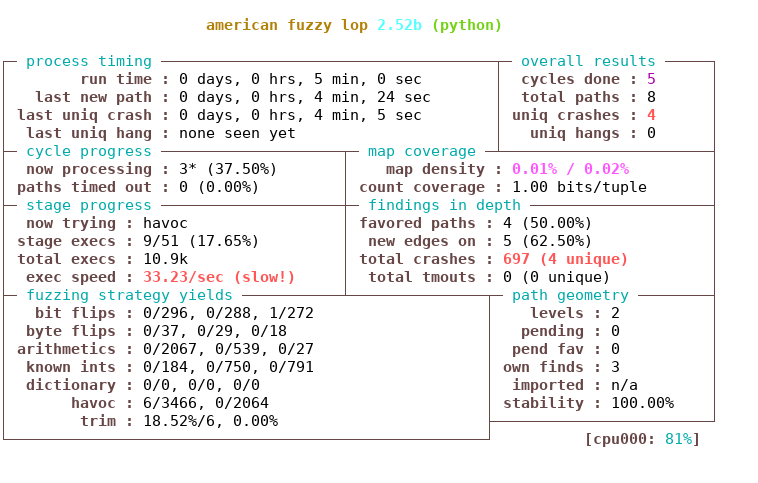
\includegraphics[scale=0.75]{images/afl-unicorn-sample.png}
  \caption{Run of afl-unicorn on the example template}
  \label{fig:aflunicornres}
\end{figure}

There are some other tools and fuzzers that can be used to test for more
vulnerabilities, fore example some of the forks of \textbf{AFL} might be have better results in efficently testing these binaries. Other tools such as LLVM, which includes a fuzzer, a memory and a addresses sanitizer and Valgrind might be used to explore areas that \textbf{AFL} is not able to test.

\end{document}
